\documentclass[11pt]{article}
\usepackage[margin=1in]{geometry}
\usepackage{amsmath,amssymb,amsthm,mathtools,mathrsfs}
\usepackage{graphicx}
\usepackage{microtype}
\usepackage[colorlinks=true,linkcolor=blue,citecolor=blue,urlcolor=blue]{hyperref}

\newtheorem{theorem}{Theorem}
\newtheorem{lemma}{Lemma}
\newcommand{\T}{\mathbb T}
\newcommand{\Pp}{\mathscr P}
\newcommand{\E}{\mathbb E}
\newcommand{\cC}{C(\T)}
\renewcommand{\thesection}{\arabic{section}.}

\title{Uniform convergence for dependent Gaussian Fourier series\\
and a sharp cotype obstruction}
\author{Candidate full answers to two questions in arXiv:2103.09579}
\date{13 August 2026}

\begin{document}
\maketitle

\noindent\fbox{\parbox{0.94\linewidth}{\textbf{Status: candidate full results,
likely valid.}  Under exactly the hypotheses of Theorem~4 in the source,
condition~(8) does imply almost-sure uniform convergence.  In contrast, the
suggested cotype-$2$ extension to general stationary Gaussian processes is
false, even within the same covariance-matrix class.}}

\section{Source questions}

Let $(\xi_n)_{n\in\mathbb Z}$ be a centered stationary proper complex
Gaussian sequence of unit variance, with
\[
 \E(\xi_n\overline{\xi_m})=\gamma(n-m),
 \qquad \E(\xi_n\xi_m)=0.
\]
Theorem~4 of Mukeru's paper assumes that, for some $b\ge0$, the matrix
\begin{equation}\label{eq:A}
 A_{nm}=|\gamma(n-m)|\,|nm|^{-b},\qquad n,m\ne0,
\end{equation}
defines a bounded operator on $\ell^2(\mathbb Z\setminus\{0\})$.  For
$f\in L^2(\T)$ it imposes
\begin{equation}\label{eq:MP}
 \sum_{|n|\ge2}\frac{1}{|n|\sqrt{\log|n|}}
 \left(\sum_{|k|\ge |n|}|\widehat f(k)|^2|k|^{2b}\right)^{1/2}<\infty.
\end{equation}
The source proves almost-sure boundedness of the associated random Fourier
series.  Remark~2 asks whether \eqref{eq:MP} gives almost-sure uniform
convergence, as in the independent case.  It also asks for an analogue of
Pisier's cotype-$2$ theorem for general stationary Gaussian processes [1].

\begin{figure}[h]
 \centering
 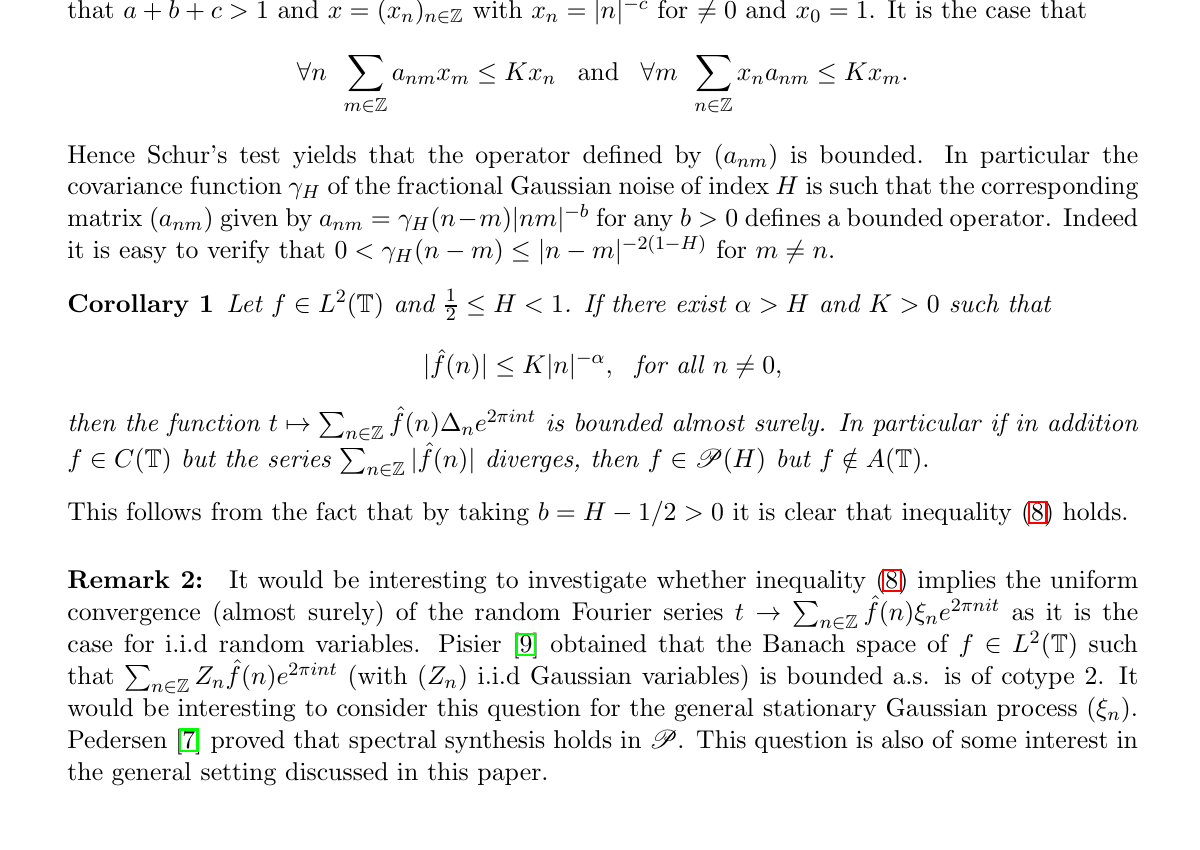
\includegraphics[width=0.97\linewidth]{figures/remark2_crop.png}
 \caption{The end of Theorem~4, its corollary, and the two questions in
 Remark~2 on page~8 of arXiv:2103.09579.}
\end{figure}

\section{Proof intuition}

The source compares the limiting dependent process with an independent
Gaussian Fourier series and concludes boundedness.  To obtain convergence,
one must compare more at once: put every difference of every two tail
partial sums into a single Gaussian process.  The matrix hypothesis controls
arbitrary finitely supported coefficient vectors, so it controls every
canonical-metric increment of this much larger process.  Gaussian comparison
then bounds the full dependent tail diameter by the independent one.

The independent comparator converges uniformly by the classical criterion
already used in the source.  Its tail diameter tends to zero in expectation.
The dependent tail diameters decrease with the starting index, so expectation
tending to zero makes their almost-sure limit zero.  This supplies precisely
the missing uniform-Cauchy conclusion.

The cotype question has a different answer.  At the extreme of perfect
dependence, $\xi_n$ is the same Gaussian for every $n$.  The corresponding
Pisier-type algebra is simply $C(\T)$, which contains $\ell_\infty^N$
uniformly and has no finite cotype.

\section{Uniform convergence}

For symmetric partial sums write
\[
 S_N(t)=\sum_{|n|\le N}\widehat f(n)\xi_ne^{2\pi int}.
\]

\begin{lemma}[coefficient domination]\label{lem:quad}
Let $K=\|A\|$.  For every finitely supported complex sequence $(c_n)$ on
$\mathbb Z\setminus\{0\}$,
\begin{equation}\label{eq:quad}
 \E\left|\sum_n c_n\xi_n\right|^2
 \le K\sum_n|c_n|^2|n|^{2b}.
\end{equation}
\end{lemma}

\begin{proof}
Set $u_n=|c_n||n|^b$.  The covariance form is nonnegative, and entrywise
absolute values followed by \eqref{eq:A} give
\[
 \E\left|\sum_n c_n\xi_n\right|^2
 \le\sum_{n,m}|\gamma(n-m)|\,|c_n|\,|c_m|
 =\langle Au,u\rangle
 \le K\|u\|_2^2.\qedhere
\]
\end{proof}

Let $(g_n)$ be independent standard proper complex Gaussians and define
\[
 Y_N(t)=\sum_{|n|\le N}\widehat f(n)|n|^b g_ne^{2\pi int},
\]
with the harmless zero-frequency convention omitted.  Condition
\eqref{eq:MP}, split into positive and negative frequencies, is the
Marcus--Pisier sufficient condition invoked in the source.  Hence $(Y_N)$
converges uniformly on $\T$ almost surely.

\begin{theorem}[affirmative answer to Remark~2]\label{thm:uniform}
Under the hypotheses of Theorem~4 of the source and condition
\eqref{eq:MP}, the partial sums $S_N$ converge uniformly on $\T$ almost
surely.  In particular the random Fourier series has a continuous version.
\end{theorem}

\begin{proof}
Define the two tail diameters
\[
 D_N^S=\sup_{M,L\ge N}\|S_M-S_L\|_\infty,
 \qquad
 D_N^Y=\sup_{M,L\ge N}\|Y_M-Y_L\|_\infty.
\]
We claim
\begin{equation}\label{eq:compare}
 \E D_N^S\le \sqrt K\,\E D_N^Y.
\end{equation}

First restrict $M,L$ to a finite range and $t$ and
$\theta\in[0,2\pi]$ to finite sets.  Consider the centered real Gaussian
process
\[
 X_{M,L,t,\theta}
 =\operatorname{Re}\!\left(e^{-i\theta}(S_M(t)-S_L(t))\right).
\]
The difference of any two of its coordinates is a finite linear combination
of the $\xi_n$.  Lemma~\ref{lem:quad} applies to that coefficient vector.
Properness gives
$\E(\operatorname{Re}Z)^2=\frac12\E|Z|^2$, so its canonical metric is
dominated by that of
\[
 \sqrt K\operatorname{Re}\!\left(e^{-i\theta}
 (Y_M(t)-Y_L(t))\right).
\]
Sudakov--Fernique comparison proves the finite-index version of
\eqref{eq:compare}.  Letting the finite range grow and using dense sets of
$t$ and $\theta$ gives \eqref{eq:compare}; the phase parameter uses
$|z|=\sup_\theta\operatorname{Re}(e^{-i\theta}z)$.

Because $(Y_N)$ converges uniformly almost surely, $D_N^Y\to0$ almost
surely.  The symmetric shells of $(Y_N)$ are independent symmetric random
elements of the separable Banach space $C(\T)$.  Its limit $Y$ is Gaussian,
so Fernique's theorem gives $\E\|Y\|_\infty<\infty$.  The Banach-valued
L\'evy maximal inequality then yields
\[
 \E\sup_N\|Y_N\|_\infty<\infty.
\]
Since $D_N^Y\le2\sup_M\|Y_M\|_\infty$, dominated convergence gives
$\E D_N^Y\to0$.  Equation \eqref{eq:compare} implies
$\E D_N^S\to0$.

Finally, $D_N^S$ decreases as $N$ increases.  Therefore
\[
 \E\left(\lim_{N\to\infty}D_N^S\right)
 =\lim_{N\to\infty}\E D_N^S=0.
\]
Thus $D_N^S\to0$ almost surely, exactly saying that $(S_N)$ is uniformly
Cauchy.  Its uniform limit is continuous.  At each fixed $t$, the source's
$L^2(\mathbb P)$ convergence identifies this limit with the stated formal
Gaussian Fourier series.
\end{proof}

\section{The cotype extension fails}

\begin{theorem}[counterexample to general cotype $2$]\label{thm:cotype}
There is a stationary proper complex Gaussian sequence, satisfying the
matrix hypothesis \eqref{eq:A} for some $b$, whose Pisier-type algebra has
no finite cotype.  Hence a general stationary-Gaussian analogue of Pisier's
cotype-$2$ conclusion is false.
\end{theorem}

\begin{proof}
Let $Z$ be one standard proper complex Gaussian and set
\[
 \xi_n=Z\qquad(n\in\mathbb Z).
\]
This sequence is stationary, $\gamma(k)=1$, and its spectral measure is the
point mass $\delta_0$.  In the source's construction the canonical process
is
\[
 X_f(t)=f(t)Z.
\]
Consequently every $f\in C(\T)$ belongs to $\Pp(\delta_0)$, and
\begin{equation}\label{eq:normeq}
 \|f\|_\infty
 \le\|f\|_{\Pp(\delta_0)}
 \le(1+2\E|Z|)\|f\|_\infty.
\end{equation}
Thus $\Pp(\delta_0)$ is isomorphic to $C(\T)$.

For each $N$, choose $N$ continuous norm-one bumps with pairwise disjoint
supports.  Their span is isometric to $\ell_\infty^N$ in the supremum norm,
and \eqref{eq:normeq} makes the distortion uniform in $N$.  If the space had
cotype $q<\infty$ with constant $C$, its coordinate vectors would give
\[
 N^{1/q}\le C\left(\E_\varepsilon
 \left\|\sum_{j=1}^N\varepsilon_je_j\right\|_\infty^q\right)^{1/q}=C,
\]
an impossibility as $N\to\infty$.

The example even satisfies \eqref{eq:A}.  If $b>1/2$, then on nonzero
indices
\[
 A_{nm}=|n|^{-b}|m|^{-b}=v_n v_m,
 \qquad v=(|n|^{-b})_{n\ne0}\in\ell^2.
\]
Thus $A=v\otimes v$ is a bounded rank-one operator.
\end{proof}

\section{Scope and novelty}
\small

Theorem~\ref{thm:uniform} answers the first question in Remark~2 under
exactly the source hypotheses.  Theorem~\ref{thm:cotype} answers the adjacent
general cotype question negatively, including inside the source's weighted
covariance class.  We do not settle the third prompt, spectral synthesis for
general $\Pp(\mu)$; the point-mass example is $C(\T)$ and gives no
obstruction there.

A bounded search on 13 August 2026 used the exact title and the terms
stationary Gaussian Fourier series, uniform convergence, cotype, and
Pisier-type algebra.  It found the source and classical background, but no
later answer to either prompt and no matching all-tail comparison.  Novelty
confidence is moderate because the affirmative argument is a short maximal
upgrade of the source's own comparison.

\medskip
\noindent\textbf{Human-review focus.}
Check that Lemma~\ref{lem:quad} applies to differences of arbitrary partial
sum coordinates; the realification in \eqref{eq:compare}; the integrability
of the independent maximal norm; and whether the cotype prompt is intended
for precisely $\Pp(\mu)$ or its equivalent polynomial completion.

\medskip
\noindent{\large\bfseries References}\par\smallskip
\noindent[1] S.~Mukeru, \emph{A generalisation of Pisier homogeneous Banach
algebra}, arXiv:2103.09579 (2021).\par
\noindent[2] M.~B. Marcus and G.~Pisier, \emph{Random Fourier Series with
Applications to Harmonic Analysis}, Princeton University Press, 1981.\par
\noindent[3] M.~Ledoux and M.~Talagrand, \emph{Probability in Banach Spaces},
Springer, 1991.

\end{document}
